\documentclass{standalone}
\usepackage{tikz,xcolor,amsmath}
\begin{document}
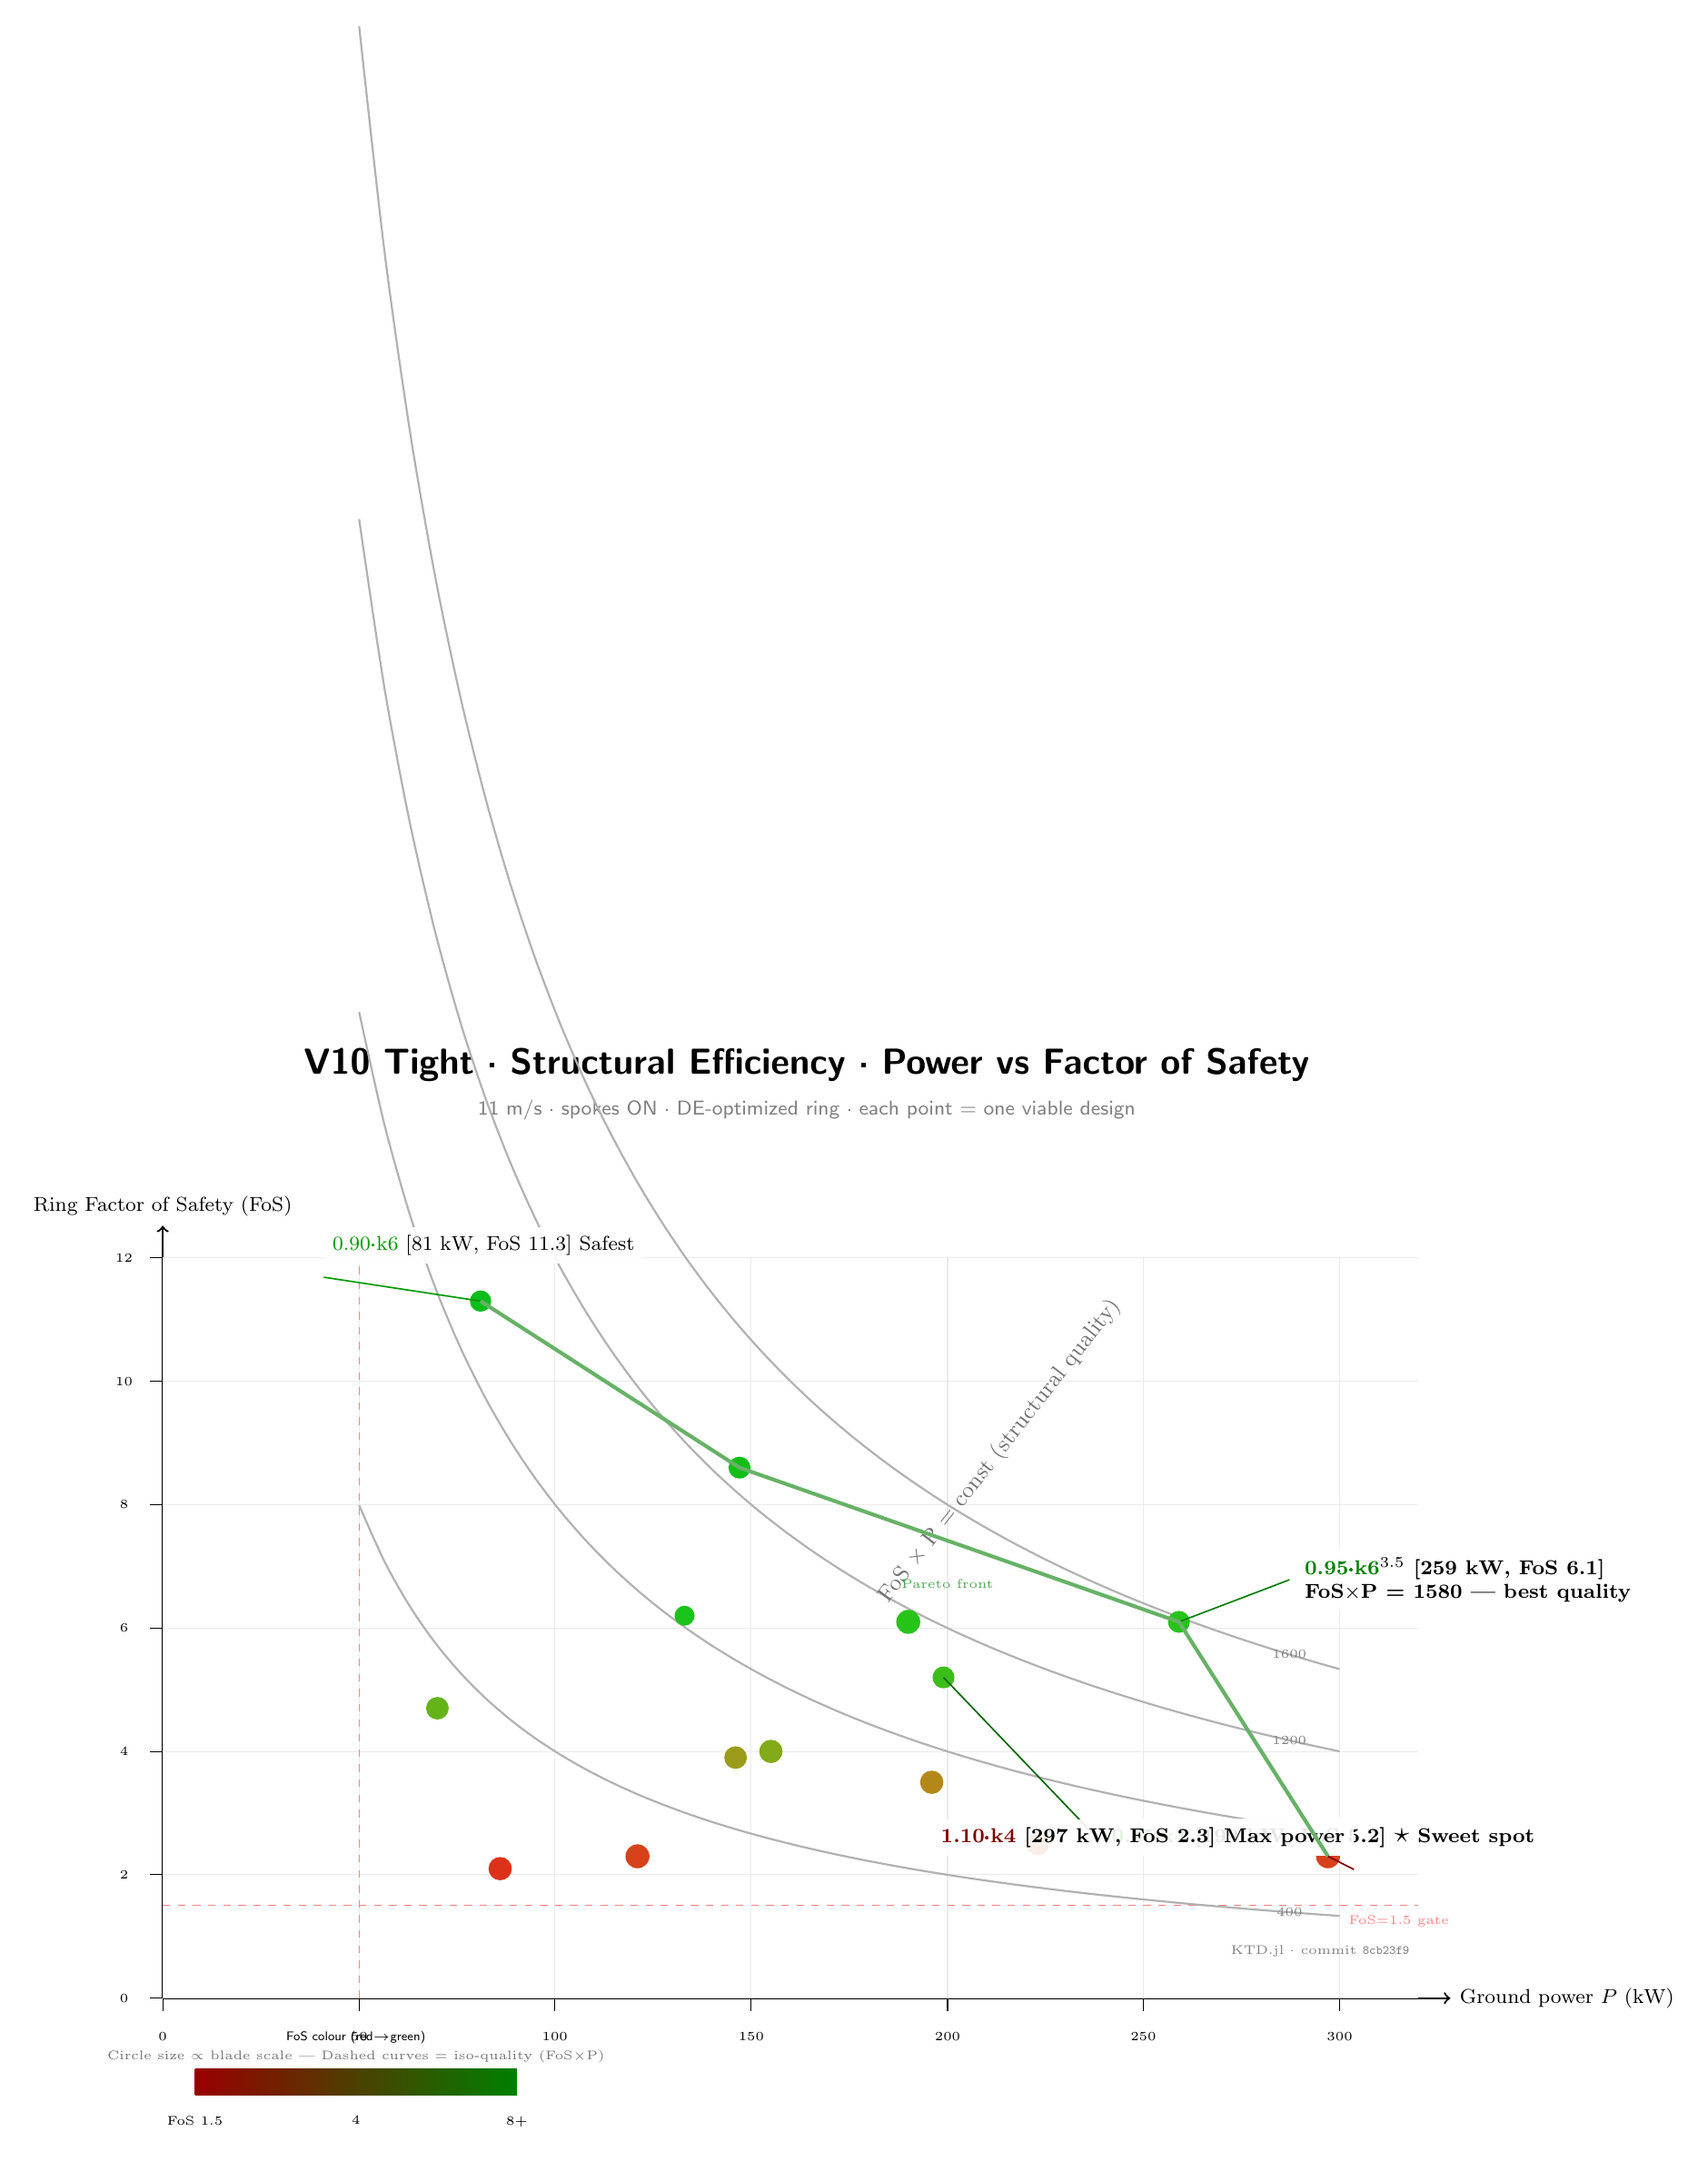
\begin{tikzpicture}[scale=0.90]

% ── Title ──
\node[font=\Large\sffamily\bfseries] at (12.0, 16.5) {V10 Tight · Structural Efficiency · Power vs Factor of Safety};
\node[font=\footnotesize\sffamily, black!50] at (12.0, 15.8) {11 m/s · spokes ON · DE-optimized ring · each point = one viable design};

% ── Axes ──
\draw[->, thick] (2.0, 2.0) -- (22.0, 2.0) node[right, font=\footnotesize] {Ground power $P$ (kW)};
\draw[->, thick] (2.0, 2.0) -- (2.0, 14.0) node[above, font=\footnotesize] {Ring Factor of Safety (FoS)};

% Grid
\foreach \p/\x in {0/2.0, 50/5.05, 100/8.09, 150/11.14, 200/14.19, 250/17.23, 300/20.28} {
  \draw[black!8] (\x, 2.0) -- (\x, 13.5);
  \draw (\x, 1.8) -- (\x, 2.0); \node[font=\tiny] at (\x, 1.4) {\p};
}
\foreach \f/\y in {0/2.0, 2/3.92, 4/5.83, 6/7.75, 8/9.67, 10/11.58, 12/13.5} {
  \draw[black!8] (2.0, \y) -- (21.5, \y);
  \draw (1.8, \y) -- (2.0, \y); \node[font=\tiny] at (1.4, \y) {\f};
}

% Gates
\draw[dashed, red!50] (2.0, 3.44) -- (21.5, 3.44);
\node[font=\tiny, red!50] at (21.2, 3.2) {FoS=1.5 gate};
\draw[dashed, red!50] (5.05, 2.0) -- (5.05, 13.5);

% Iso-quality curves — darker
\foreach \q/\lbl in {400/400, 800/800, 1200/1200, 1600/1600} {
  \draw[black!30, line width=0.8pt, domain=5.05:20.28, samples=40, smooth] 
    plot (\x, {2.0 + (\q/((\x-2.0)*320/19.5))*11.5/12});
  \pgfmathsetmacro{\ly}{2.0 + (\q/((19.5-2.0)*320/19.5))*11.5/12}
  \node[font=\tiny, black!50] at (19.5, \ly) {$\lbl$};
}
\node[font=\small, black!55, rotate=52] at (15.0, 10.5) {FoS $\times$ P = const (structural quality)};

% ── Helpers ──
\def\px#1{2.0 + #1/320*19.5}
\def\py#1{2.0 + #1/12*11.5}
\def\siz#1{2.0 + #1*3.0}

% ═══════════════════════════════════════
% FoS colors (red→green spectrum)
% ═══════════════════════════════════════
\definecolor{fosA}{RGB}{220,50,25}
\definecolor{fosB}{RGB}{215,65,25}
\definecolor{fosC}{RGB}{200,100,25}
\definecolor{fosD}{RGB}{180,135,25}
\definecolor{fosE}{RGB}{155,155,25}
\definecolor{fosF}{RGB}{130,170,25}
\definecolor{fosG}{RGB}{100,180,25}
\definecolor{fosH}{RGB}{60,190,25}
\definecolor{fosI}{RGB}{40,195,25}
\definecolor{fosJ}{RGB}{25,195,25}
\definecolor{fosK}{RGB}{20,190,25}
\definecolor{fosL}{RGB}{10,190,28}

% ═══════════════════════════════════════
% DATA POINTS
% ═══════════════════════════════════════
\fill[fosL] (\px{81},  \py{11.3}) circle (\siz{0.90} pt);
\fill[fosK] (\px{147}, \py{8.6})  circle (\siz{0.95} pt);
\fill[fosJ] (\px{133}, \py{6.2})  circle (\siz{0.80} pt);
\fill[fosI] (\px{259}, \py{6.1})  circle (\siz{0.95} pt);
\fill[fosI] (\px{190}, \py{6.1})  circle (\siz{1.10} pt);
\fill[fosH] (\px{199}, \py{5.2})  circle (\siz{0.95} pt);
\fill[fosG] (\px{70},  \py{4.7})  circle (\siz{1.00} pt);
\fill[fosF] (\px{155}, \py{4.0})  circle (\siz{1.05} pt);
\fill[fosE] (\px{146}, \py{3.9})  circle (\siz{1.00} pt);
\fill[fosD] (\px{196}, \py{3.5})  circle (\siz{1.05} pt);
\fill[fosC] (\px{223}, \py{2.5})  circle (\siz{1.00} pt);
\fill[fosB] (\px{297}, \py{2.3})  circle (\siz{1.10} pt);
\fill[fosB] (\px{121}, \py{2.3})  circle (\siz{1.10} pt);
\fill[fosA] (\px{86},  \py{2.1})  circle (\siz{1.05} pt);

% ═══════════════════════════════════════
% KEY DESIGN LABELS — positioned closer to points
% ═══════════════════════════════════════

% Highest quality (top-right callout)
\draw[green!50!black, line width=0.6pt] (\px{259}, \py{6.1}) -- (19.5, 8.5);
\node[font=\footnotesize\bfseries, anchor=west, align=left, fill=white, fill opacity=0.9, text opacity=1] at (19.6, 8.5) {\textcolor{green!50!black}{0.95·k6}$^{3.5}$ [259 kW, FoS 6.1]\\FoS$\times$P = 1580 — best quality};

% Sweet spot — place label near the point
\draw[green!40!black, line width=0.6pt] (\px{199}, \py{5.2}) -- (16.5, 4.5);
\node[font=\footnotesize\bfseries, anchor=west, fill=white, fill opacity=0.9, text opacity=1] at (16.6, 4.5) {\textcolor{green!40!black}{0.95·k4} [199 kW, FoS 5.2] {\large$\star$} Sweet spot};

% Max power — near the point
\draw[red!50!black, line width=0.6pt] (\px{297}, \py{2.3}) -- (20.5, 4.0);
\node[font=\footnotesize\bfseries, anchor=south east, fill=white, fill opacity=0.9, text opacity=1] at (20.5, 4.2) {\textcolor{red!50!black}{1.10·k4} [297 kW, FoS 2.3] Max power};

% Safest
\draw[green!60!black, line width=0.6pt] (\px{81}, \py{11.3}) -- (4.5, 13.2);
\node[font=\footnotesize, anchor=south west, fill=white, fill opacity=0.9, text opacity=1] at (4.5, 13.4) {\textcolor{green!60!black}{0.90·k6} [81 kW, FoS 11.3] Safest};

% Pareto front
\draw[green!50!black!60, line width=1.5pt] 
  (\px{81}, \py{11.3}) -- (\px{147}, \py{8.6}) -- (\px{259}, \py{6.1}) -- (\px{297}, \py{2.3});
\node[font=\tiny, green!50!black!70, above] at (\px{200}, \py{6.5}) {Pareto front};

% ═══════════════════════════════════════
% COLOR BAR + LEGEND
% ═══════════════════════════════════════
\shade[left color=red!60!black, right color=green!50!black] (2.5, 0.5) rectangle (7.5, 0.9);
\node[font=\tiny, below] at (2.5, 0.3) {FoS 1.5};
\node[font=\tiny, below] at (5.0, 0.3) {4};
\node[font=\tiny, below] at (7.5, 0.3) {8+};
\node[font=\tiny\sffamily, above] at (5.0, 1.15) {FoS colour (red$\rightarrow$green)};

\node[font=\tiny, black!55] at (5.0, 1.1) {Circle size $\propto$ blade scale | Dashed curves = iso-quality (FoS$\times$P)};

\node[font=\tiny, black!50, anchor=south east] at (21.5, 2.5) {KTD.jl · commit \texttt{8cb23f9}};

\end{tikzpicture}
\end{document}
